% !TEX root = ./thesis.tex

\chapter{Evaluation}
\label{ch:eval}

Finding a definite good evaluation method for unsupervised models is a long-standing and inherent problem \cite{Li2015}. In this section we describe our evaluation techniques along with data collection process. We introduce two task-independent metrics to evaluate the qualities of the extracted manifold. Further we discuss possible applications of the model to real-world data.


\section{Evaluation data}
\subsection{Data collection}

Access to large amount of training data is crucial for applying deep learning models.
Successes of deep learning on image recognition and segmentation tasks can be attributed to existence of large research datasets as ILSVRC and Places365 \cite{ILSVRC15, Zhou2016} containing millions of labeled images.
Machine translation, NLP tasks \cite{Karpathy2014, Kim2014} often rely on low-dimensional word embedding models.
Such models, as for example as word2vec or Glove \cite{Mikolov2013, pennington2014glove}, are trained on terabytes of textual data.
Deep reinforcement models might use existing gaming engines to generate required training data "on the go".
As, for example Google DeepMind team uses Atari 2D games to generate data for Q-learning \cite{Mnih2013}.

For the purpose of this research we collect visual data using the ViZDoom AI research platform \cite{Kempka2016}.
ViZDoom is a Doom-based platform for reinforcement learning.
It provides access to raw visual data from the Doom gaming engine.
Doom is a first-person shooter (FPS) computer game utilizing 3D graphics.
In context of our research the ViZDoom platform allows automatic visual data generation and collection.
Example of the output image is shown on figure \ref{fig:doom}.

We created multiple \texttt{Doom II} maps specifically for our task using the Slade \cite{Slade3} software.
Created maps provide high diversity of textures for better discrimination between images, captured from different positions on the map.
Other reason for diverse structures on the map is to explicitly brake symmetry of the map.
Symmetric maps look alike from different player positions which leads to entangled manifolds in feature space.
Such position tend to be encoded with the same values of sparse features.
This represents a difficulty for evaluation and comparison of quality of sparse features.

We record multiple movement trajectories on each map.
More specifically, we record 10000-300000 consecutive images of unstructured movement of the player on the map for training purposes.
In addition to that, we record movement along well defined structured trajectories as a "circle" or an "eight" for model evaluation and comparison of quality of extracted features.


\begin{figure}
\centering
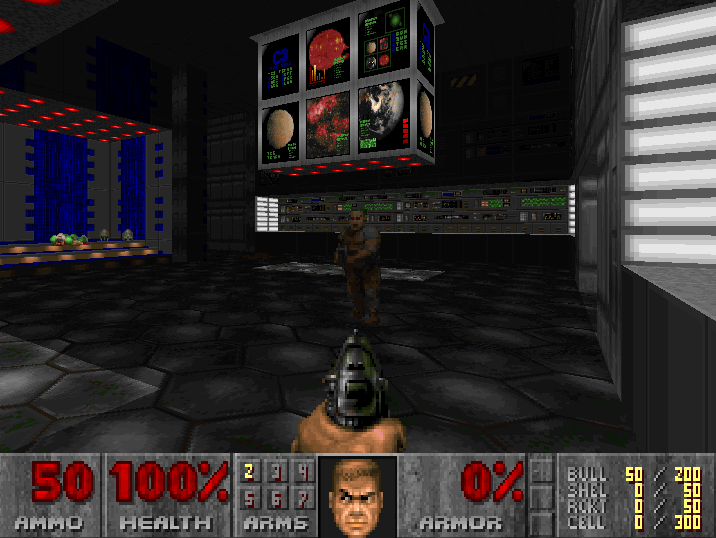
\includegraphics[width=.80\textwidth]{doom.png} %{CS0031}
\caption{Example of \texttt{Doom II} image collected with ViZDoom \cite{Kempka2016}.}
\label{fig:doom}
\end{figure}

\subsection{Dataset description}

We collect multiple sets of visual data with varying complexity of players movement.
We can specify next 3 classes of trajectories used either for training or evaluation:
\begin{itemize}
  \item Continuous closed trajectory without intersection. A circular movement is one example of such trajectory.
  \item Continuous closed trajectory with intersection. An \text{eight} is an example of such trajectory.
  \item Continuous random movement across the environment (map).
\end{itemize}

Furthermore, we introduce multiple complexity levels of movement across trajectories by reducing degrees of freedom of such movements:
\begin{itemize}
  \item Most restricted. Only movement along a single axis at a time is possible. This category includes movements across rectangular trajectories while maintaining fixed direction of the view or changing the direction of the view while standing still. This category provides includes trajectories of the lowest complexity.
  \item Less restricted. Multiple degrees of freedom at a time allowed. For example, movement along multiple axis facing one direction or forward movement while changing the direction of the view.
  \item Free movement across the map with no restrictions.
\end{itemize}


\subsection{Data format}

We collect RGBD images from the 3D engine. Each image has resolution of 160 by 120 pixels. Each pixel is describe by 3 color channels and a single distance channel. Each channel can take a discrete value between 0 and 255 including. This format results in 76800 dimensional inputs.


\section{Predictive evaluation} \label{ss:score}

Evaluation of the performance of unsupervised models is inherently difficult.
Discriminative models typically use well-defined metrics with clear quantifiable outputs, as classification accuracy, F-measure etc. Unsupervised models generally have no access to such metrics.
Solutions for some under-defined objectives, as finding image super-resolution or generating new data samples, can be evaluated by involving manual human grading, which is costly and time-consuming \cite{Dahl2017, Goodfellow2014}.
Other models rely on the primary learning objective, which is not necessarily representative of the actual model performance. As, for example, minimizing MSE for image comparison can result in low-quality blurry results, or matching certain characteristics of natural probability distribution in a generative process does not guarantee realistically looking generated data \cite{Li2015, Mathieu2015}. At last, some unsupervised learning techniques can be evaluated through performance on real world tasks by showing, that results of unsupervised learning can improve performance of discriminative models. For example, reusing network weights of denoising and contractive autoencoders led to improved classification results \cite{Rifai2011, Vincent2010}, as well reusing weights of word embeddings \cite{NIPS2013_5021} led to increased performance on a number of natural language processing tasks.

In context of this work we would like to have access to a concise measure for comparison of model designs.
Primary objective of an autoencoder -- good reconstruction of the input image -- is not very descriptive, since it makes no assumption about the spatial characteristics of the extracted features. Nevertheless, we provide our reconstruction loss values with the experiments.

We are going to use \textit{predictive score} as a main mean of model comparison from perspective of spatial feature extraction. With the predictive objective we would like to evaluate the quality of extracted spatial features. We do that by considering local resemblance of the manifold to an euclidean space. But, since we are working with unlabeled data another assumption is required. Namely, for any trajectory of actors movement we expect, that the best approximation of the transition between current and next step to be equivalent to the transition between previous and current step (when only last two frames are available for performing the prediction). We, therefore try to predict spatial position of the player on the next step on the manifold calculating it as $\hat{x}_{t+1} = x_t + (x_t- x_{t-1})$. Figure \ref{fig:m_pred} illustrates the process.
Since different models have different deformations of manifold space and, therefore, might differ in terms of absolute values of the $L_2$ loss between predicted and actual location $L_2(\hat{x}_{t+1}, x_{t+1})$, we use relative improvement as a reference. We compare the improvement of prediction over a naive prediction $\tilde{x}_{t+1} = x_t$. We therefore define predictive metric as follows:
\begin{equation}
  \begin{aligned}
  &P_{L2}(X) = \frac{1}{N-2}\sum^{N-1}_{i=2}{f(L_2(\hat{x}_{i+1}, x_{i+1})}, {L_2(x_i, x_{i+1}))}\\
  &f(x, y) = max(0, \frac{y-x}{y}) \text{ note: } f(x, y) \in [0, 1]
  \end{aligned}
\end{equation}
where $N$ is a number of inputs in the validation set. Note, that $P_{L2}(X) \in [0, 1]$ and 1.0 indicates perfect prediction of the next frame at each moment in time; 0.0 average prediction to be worse than naive prediction. Prediction is possible only for elements starting from the 3rd, therefore first two images do not contribute to the score.

Note, that similar technique is used as a model regularization. Yet, predictive regularization is applied as a reconstruction error and does not have direct effect on the predictive score. For example, an decoder of large enough capacity can have very low reconstruction error of both actual encoding $x_{t+1}$ and predictive encoding $\hat{x}_{t+1}$, but low score of predictive evaluation. This can happen when two prototypes in the embedding space $x_{t+1}$ and $\hat{x}_{t+1}$ have distinct difference, but are still reconstructed as alike images. This case can be explained by overfitting in the decoder network.

To counter high sensitivity of the $L_2$ error function to outliers we also calculate another flavor of the described evaluation: \textit{binary predictive score}. The total $L_2$ loss value on the complete validation set can increase sharply with presence of outliers. In this case, while overall quality of the manifold might have desired properties for majority of the inputs, it can still produce high validation error. This can happen since $L_2$ error does not take into account varying density of the manifold. To counter that, we introduce a similar simplified version of predictive score, namely producing its binary form. Binary predictive score simply compares the distance between \textit{naive prediction} naive and estimate of the future frame and the prediction calculated by the previous 2 frames.

\begin{equation}
  \begin{aligned}
  & P_{NN}(X) = \frac{1}{N-2}\sum^{N-1}_{i=2}{g  \big( L_2(\hat{x}_{i+1}, x_{i+1})} - {L_2(x_i, x_{i+1}) \big) },\\
  & g(x) = \begin{cases} 1, & \mbox{if } x > 0 \\ 0, & \mbox{if } x \leq 0 \end{cases}
\end{aligned}
\end{equation}
 Value of $P_{L2}(X)$ belongs to interval $[0, 1]$ and 1.0 indicates that calculated prediction for each point was better than naive prediction; 0.0 indicates that no predicted value was better than naive prediction. Perfect score might not be achievable even for some trajectories.

\subsection{Preserving nearest neighbor relation}

Another key characteristic of the desired encoding function is high interpretability of the feature manifold.
Interpretability itself is a loosely defined characteristic. Yet, we propose an evaluation score, that should asses some features of an interpretable spatial manifold. Namely, we argue, that less entangled manifold provide grater interpretability and are more visually appealing. As a proxy measure of such quality we propose exploring nearest-neighbor relation in the input data. We expect, that on a smooth and dense manifold subsequent video frames will be closer to each other than to more remote frames. We therefore can measure, how many subsequent frames remain nearest neighbor in the manifold space. We expect such a characteristic degrade with more entangled and less smooth manifolds.



\begin{equation}
  \begin{aligned}
  & P_{\tau}(X) = \frac{1}{N-2}\sum^{N-1}_{i=2}{\tau  \big(i, m_i, n_i) },\\
  & \tau(i, m, n) =
\begin{cases}
  1, & \mbox{if } (i-1) \in \{m, n\}  \mbox{ and }  (i+1) \in \{m, n\}  \\
  0, & \mbox{if } (i-1) \notin \{m, n\}  \mbox{ and }  (i+1) \notin \{m, n\} \\
  0.5, & \mbox{otherwise }
\end{cases}
\end{aligned}
\end{equation}
where $m_i, n_i$ are indexes of top-2 nearest neighbors of element $i$.  $P_{\tau}(X)$ can take values in interval $[0, 1]$ and 1.0 means that every nearest frame at every time stamp $i$ is the nearest neighbor of the current frame in the embedding space. Value 1.0 might not be achievable, depending on the trajectory.


\section{Model comparison}

In this section we evaluate proposed models. We analyze qualities of the different models in terms of our evaluation scores. We compare performance on datasets of various complexities and analyze sensitivity to different kinds of regularizations.

\subsection{Backbone model comparison}

As a first experiment we would like to asses model behavior on a simple concept, that can be easily understood visually. For that purpose we stick low dimensional encoding in percept able 3D space. This limitation leaves us in the domain of low-complexity trajectories, that depend only on few components. Since one degree of freedom - vertical movement of players view during horizontal motion - is taken, we choose a dataset that explores only 2 degrees of freedom. We also choose a simplest type of trajectory to observe behavior on a trivial task.

First experiment is performed on a closed trajectory with intersections 'eight' that allows only movements along the axis. Player always faces the same direction, therefore we can expect components, describing direction of the view to remain fixed. Following the trajectory player makes several steps along the already visited path (see figure \ref{fig:model_reco}$(a)$). In total, dataset contain 13680 sequential images that corresponds to 3 passes along the trajectory. With this trajectory would like to asses next qualities of the embedding space:
\begin{enumerate}
  \item tractable continuous changes in the embedding over time;
  \item presence or absence of key elements of the trajectory: direction changes;
  \item existence of intersections and coherence of the intersections to the actual trajectory;
  \item visual recognizability of the trajectory in the embedding.
\end{enumerate}

Results of the experiments for 3 backbone models are shown on figure \ref{fig:model_reco}. Metrics of section \label{fig:model_reco} are calculated and mentioned in table \ref{tab:3demb}.


\begin{table}
\begin{center}
    \begin{tabular}{| l | l | l | l | l |}
    \hline
    Model  &  $P_{L2}$    &  $P_{\beta}$     &  $P_{\tau}$ &  $L_{reco}$ \\ \hline
    Fully Connected	 AE  & 0.498 & 0.728 & 0.750 & 54.40        \\
    CNN AE 	 & 0.374 & 0.632 & 0.780 & 49.60        \\
    What-Where AE 	   & 0.000 & 0.403 & 0.623 & 1.50         \\ \hline
    \end{tabular}
\end{center}
  \caption{Comparison of 3 backbone architecture performance on an artificial low-complexity trajectory. Scores   $P_{L2}$, $P_{\beta}$, $P_{\tau}$ are described in section \ref{ss:score} (higher is better). Reconstruction error $L_{reco}$ indicates quality of the image produced by the autoencoder (lower is better).}
  \label{tab:3demb}
\end{table}

\begin{figure}[t!]
	\centering
	\subfigure[Reference \textit{trivial} trajectory]{
  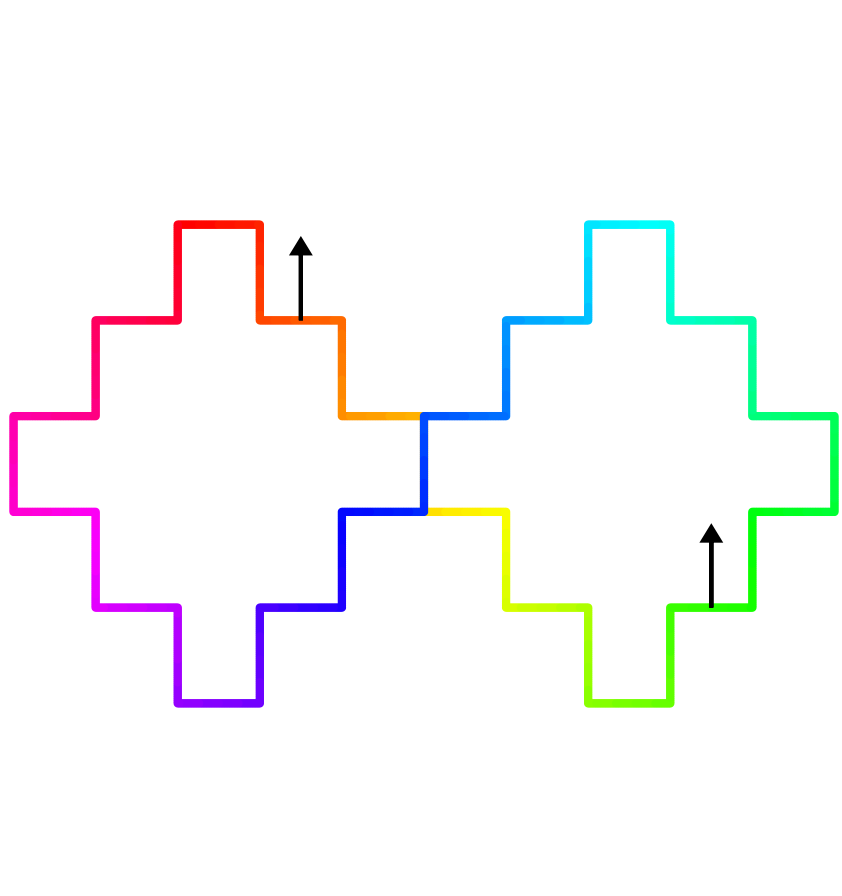
\includegraphics[width=.45\textwidth]{cmp2/tr1.png}
	}
	\subfigure[Embedding with a Fully connected AE.]{
		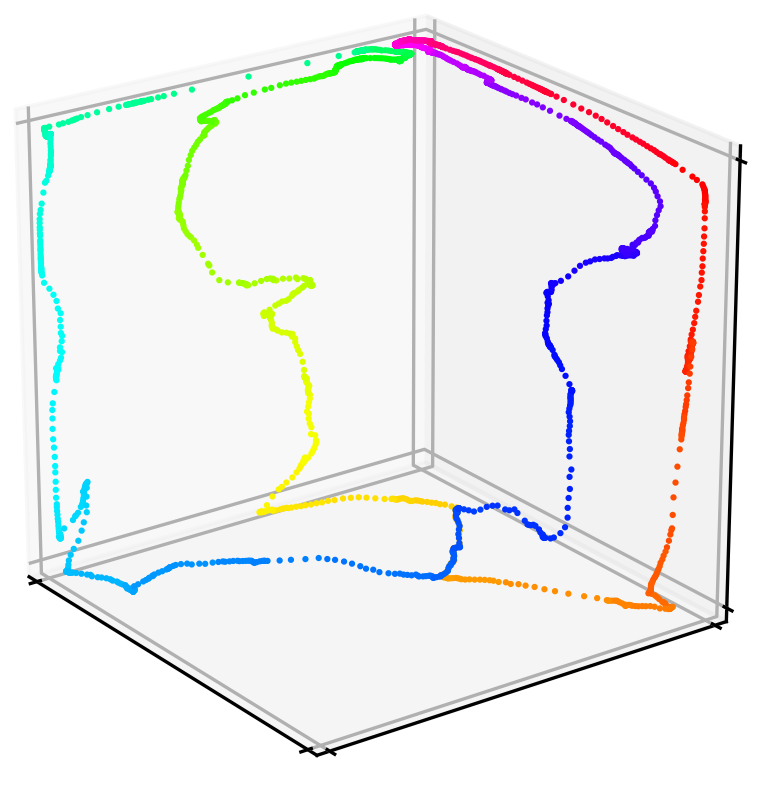
\includegraphics[width=.45\textwidth]{cmp2/fc_3.png}
	}\\
	\subfigure[Embedding with a Convolutions AE.]{
    	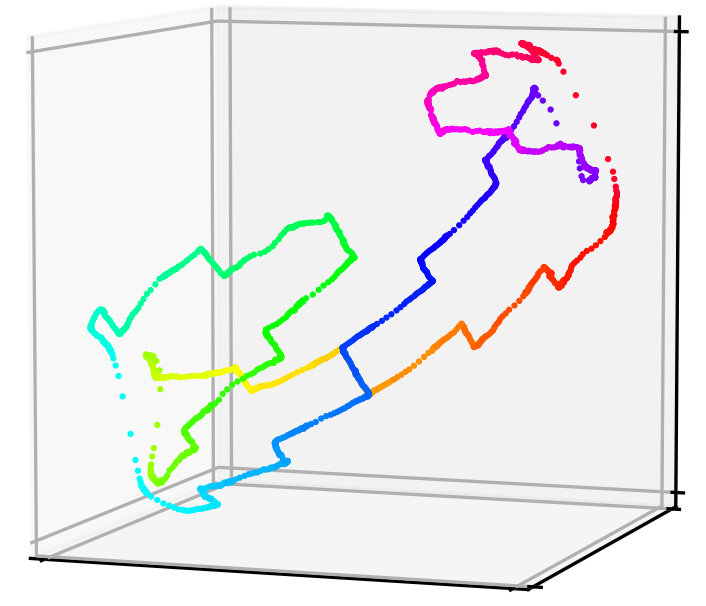
\includegraphics[width=.45\textwidth]{cmp2/cnn_3.png}
	}
	\subfigure[Embedding with the What-Where AE.]{
    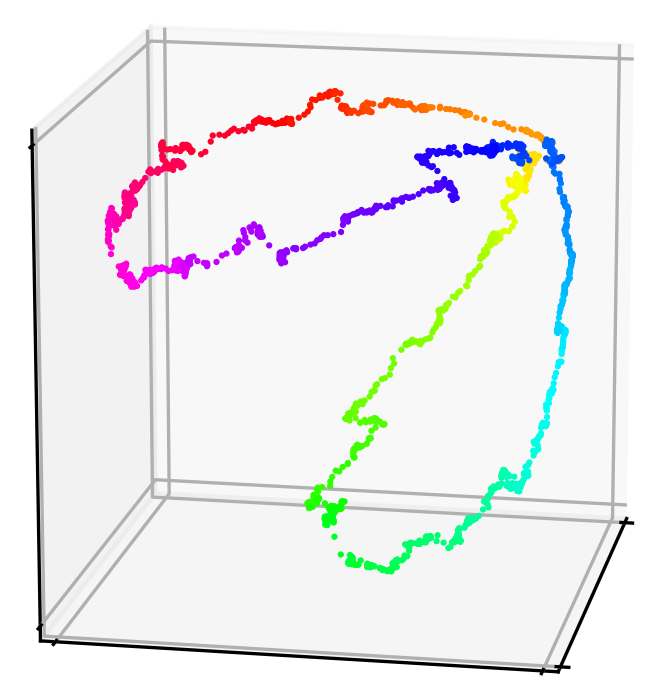
\includegraphics[width=.45\textwidth]{cmp2/ww_3.png}
	}
    	\caption{Embedding a trivial closed self-intersecting trajectory $(a)$ with 2 degrees of freedom using reference models $(b, c, d)$ in a 3-dimensional space. Subsequent frames of the input image sequence are encoded in similar colors to indicate temporal relation between visually disconnected discrete inputs in the embedding space. Color is consistent among the models and corresponds to same points of the trajectory.}
    	\label{fig:model_reco}
\end{figure}

From perspective of the metrics described in section \ref{ss:score} models distinguish sharply. What-Where AE model, while yielding best reconstructions, produced lowest quality embedding space. Average prediction were of a worth quality than using current position as an estimator and only 40\% of the predictions were closer to the actual position of the next frame than current frame. All models were able to maintain more than 63\% of nearest neighbor relations between frames with Convolutional model showing slightly better results than others. Fully connected model produced embedding of the highest predictive power, showing best predictive scores $P_{L2}, P_{\beta}$.

Visual harassment of the embedded trajectories \label{fig:model_reco} shows, that all models were able to preserve somewhat continuous form of the trajectory. All models were able to maintain model elements as intersection and direction changes in some form. Comparing embedding spaces we can see, that embedding produces by What-Where AE falls behind the other models. This observation is coherent with numerical scores calculated above. What-Where AE were able to produce the least complex manifold structure among 3 models. Yet, we are going to ignore this model in future experiments, since with higher dimensional and more complex concepts performance drops sharply and visual assessment is not longer possible without using specialized visualization techniques.

Convolutional model produced the most visually pleasing results. It falls behind the fully-connected model in terms of the synthetic scores, but saw steady improvement with the increase of network capacity (namely, increased size of the feature maps in the layers) and were only limited by our computational resources. Convolutional model was able maintain visually parallel lines of the input trajectory and maintain larger distance between parts of the trajectory. Fully convolutional model appears to spread the trajectory embedding along the surface of the embedding space.

\subsection{Effects of regularization}

In this subsection we try to analyze effects of the regularization on the qualities of the extracted manifold. This time we use a more complex trajectory. Since visual assessment is not a goal of this experiment, we can safely use higher dimensional embedding space. For this experiment we use a natural closed trajectory with single intersection "eight" where player always faces the direction of the movement. This trajectory corresponds to a more natural type of players movement and involves more complex between-frame transformations caused by changing the direction of the view. Sample of the trajectory and regularization are shown on figure \ref{fig:model_param}.

\begin{table}
\begin{center}
    \begin{tabular}{| l | l | l | l | l | l | l | l |}
    \hline
    \multirow{2}{*}{Regularization}      &\multicolumn{3}{|c|}{Parameters} & \multicolumn{4}{|c|}{Scores}  \\   \cline{2-8}

     & $\alpha$ & $\beta$ & $\gamma$    &  $P_{L2}$ & $P_{\beta}$ & $P_{\tau}$ & $L_{reco}$ \\ \hline

		No regularization 	& 0    & 0 & 0 & 0.000 & 0.418 & 0.617 & 60.64 \\ \hline
		Predictive          & 100  & 0 & 0 & 0.052 & 0.614 & 0.738 &  \textbf{57.46} \\
		Denoising           & 0    & 0.0005 & 0 & 0.078 & 0.648 & 0.750 & 61.84 \\
		Distance            & 0    & 0 & 50 & 0.063 & 0.623 & 0.739 & 59.62 \\ \hline
    Predictive and denoising 	& 100    & 0.0005 & 0 & 0.069 & 0.653 & 0.751 & 61.57 \\
    Predictive and distance  & 100    & 0 & 50 & \textbf{0.591} & \textbf{0.909} & \textbf{0.912} & 61.19 \\
    Denoising and distance  & 0    & 0.0005 & 50 & 0.081 & 0.649 & 0.758 & 60.16 \\ \hline
    All 3 & 100    & 0.0005 & 50 & \textbf{0.591} & 0.905 & 0.911 & 62.04 \\ \hline
    \end{tabular}
\end{center}
  \caption{Regularization effects.}
  \label{tab:8emb}
\end{table}

\begin{figure}[t!]
	\centering

	\subfigure[Reference \textit{eight} trajectory]{
  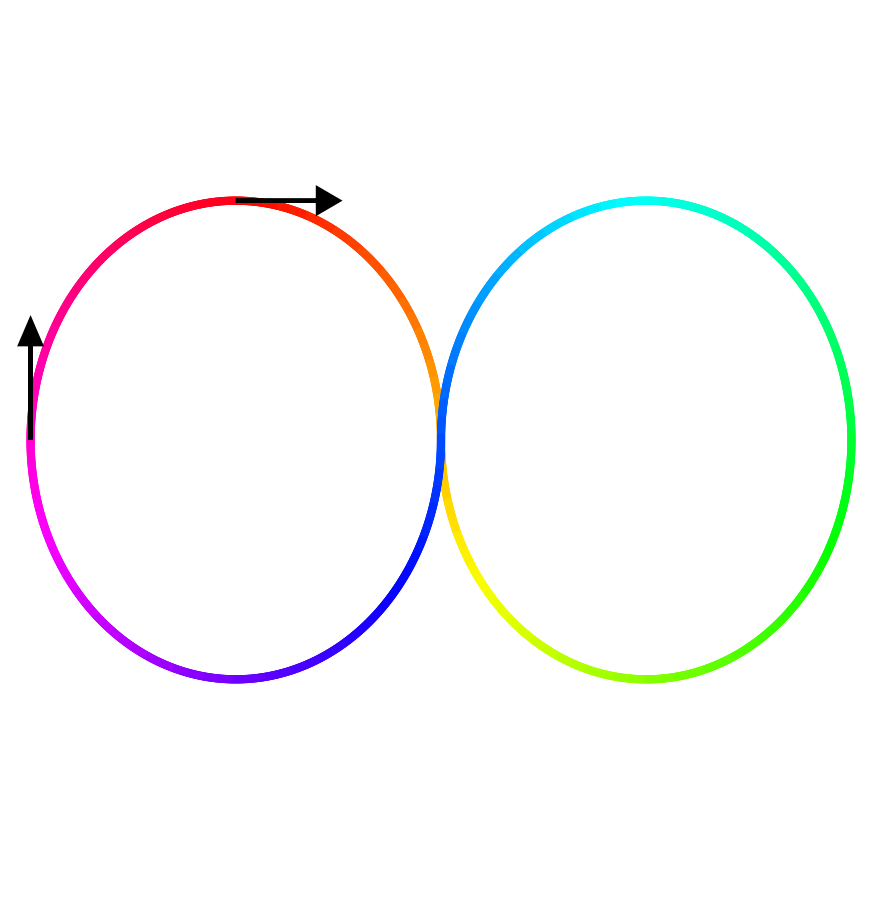
\includegraphics[width=.45\textwidth]{cmp3/tr2.png}
	}
	\subfigure[Embedding with a CNN AE.]{
		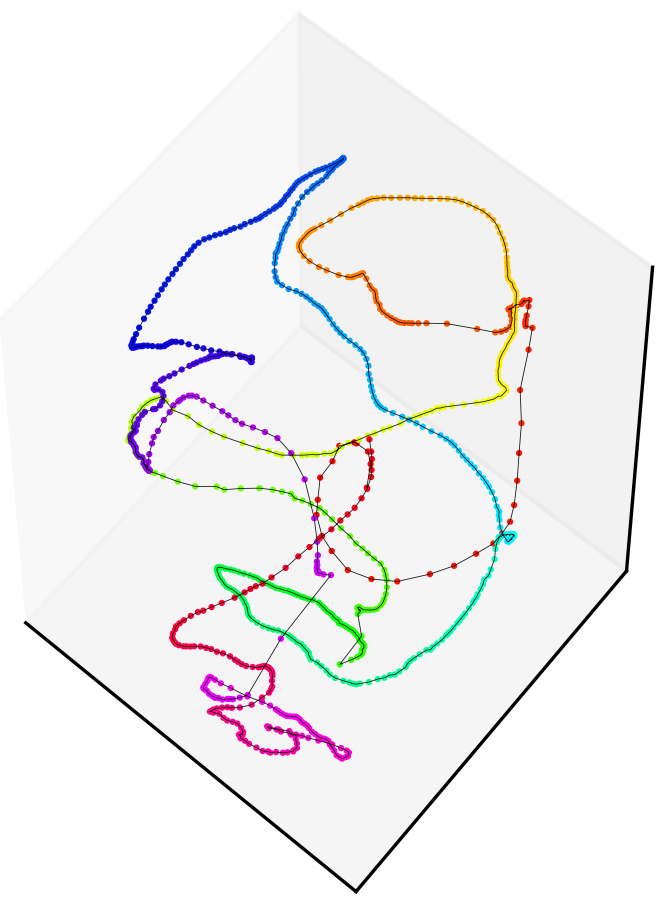
\includegraphics[width=.45\textwidth]{cmp3/cnn4_2.png}
	}\\
  \subfigure[Frames from the \textit{Eight} self-intersection trajectory.]{
    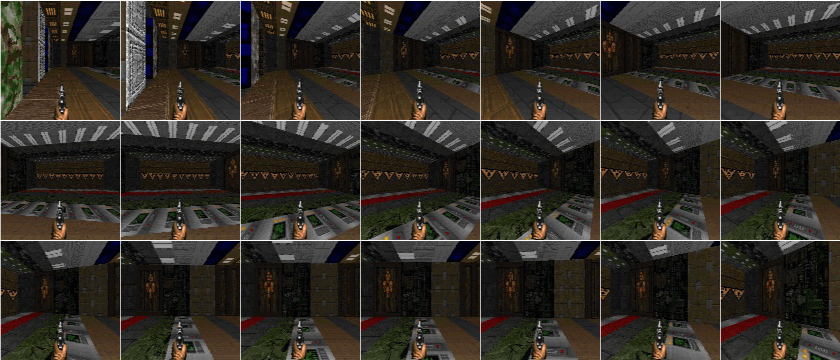
\includegraphics[width=.90\textwidth]{sprite2.png}
  }\\
    	\caption{Embedding a closed self-intersecting trajectory $(a, c)$ in a lower dimensional space using CNN AE. Black arrows on the reference trajectory indicate the direction of the player's view. Each embedding frame is visualized as time-colored point, subsequent frames are connected by a black line.}
    	\label{fig:model_param}
\end{figure}

Our experiments revealed, that models, based on a fully connected configuration show either similar or worth results comparing to CNN for more complex datasets while following the same trends as below. We therefore only provide results for better performing convolutional models.

We tested our training method on 8 possible configurations of the regularization. Best values of the error weight were selected with a grid search and has been fixed throughout the training. Model without any regularization showed
no improvement according to the predictive metric and binary predictive metric is well below 50\%. Yet, model was able to preserve 61.7\% of nearest neighbor relations.

When using a single type of regularization all 3 methods showed comparable results. Using a single regularization allows 5 to 8\% more accurate prediction of the next position on the manifold. Prediction of the future frame was more accurate than naive prediction in around 61-65\% of the time. In terms of reconstruction quality predictive regularization allowed to archive significant improvement over the non-regularized model. Interestingly, applied alone, denoising regularization showed the best results among the 3.

Among 3 models utilizing 2 types of regularization all showed at least marginal improvement over models with single regularization technique with "Predictive and distance" regularized model sharply outperforming all the others. "Predictive and distance" showed 59\% improvement in accuracy of future position prediction with 91\% of predictions being more accurate than naive prediction. It also managed to maintain 91\% of nearest neighbor relations in the embedding space.Reconstruction accuracy decreased.

Adding Denoising regularization to the best model so far did not have any significant effect as shown in the last line of the table \ref{tab:8emb}. We therefore take the combination of predictive and distance regularization as the main configuration of the model.


\subsection{Dataset complexity}

In this section we test our low-dimensionality embedding method on a large realistic dataset. We further evaluate test model on a trajectory which is not present in the training set, although recorded on the same map. We use a long continuous trajectory on a single \texttt{Doom II} map containing 300000 training images.
As validation we use a "circle" and an "eight" continuous trajectory similar to one described in previous experiment.
Data collection method guaranties, that while train and validation trajectories might contain similar or identical images, this images do not appear in duplicated subsequences i.e. if $t_i = v_j$ than $t_{i+1} \neq v_{j+1}$ for $\forall i \leq |T|$, where $T, V$ are validation and training sets. This constrain allows us to state, that even if continuity of training trajectory is imposed explicitly by the predictive regularization and only indicates overfitting, validation data shall not have the same quality.

\begin{table}
\begin{center}
    \begin{tabular}{| l | l | l | l | l |}
      \hline
     Model configuration  &  $P_{L2}$ & $P_{\beta}$ & $P_{\tau}$ & $L_{reco}$ \\ \hline
     16c3-p2-32c3-p2-32c3-p2-16c3-f3     & 0.000 & 0.222 & 0.356 & 69.98 \\
     16c3-p2-32c3-p2-32c3-p2-16c3-f100-f3 & 0.000 & 0.246 & 0.376 & 66.72 \\
     16c3-p2-32c3-p2-32c3-p2-16c3-f250-f3 & 0.000 & 0.249 & 0.387 & 66.72 \\
     16c3-p2-32c3-p2-32c3-p2-16c3-f250-f4 & 0.000 & 0.225 & 0.474 & 65.08 \\
     16c3-p2-32c3-p2-32c3-p2-16c3-f8      & 0.000 & 0.091 & 0.588 & 64.30 \\
     16c3-p2-32c3-p2-32c3-p2-16c3-f80-f8  & 0.000 & 0.149 & 0.587 & 57.09 \\ \hline
     \end{tabular}
\end{center}
  \caption{Validation performance of different model configurations on a large training set with multiple degrees of freedom.}
  \label{tab:large}
\end{table}

\begin{figure}[t!]
	\centering
	\subfigure[Trivial \textit{eight} trajectory as on figure \ref{fig:model_reco}(a) ]{
  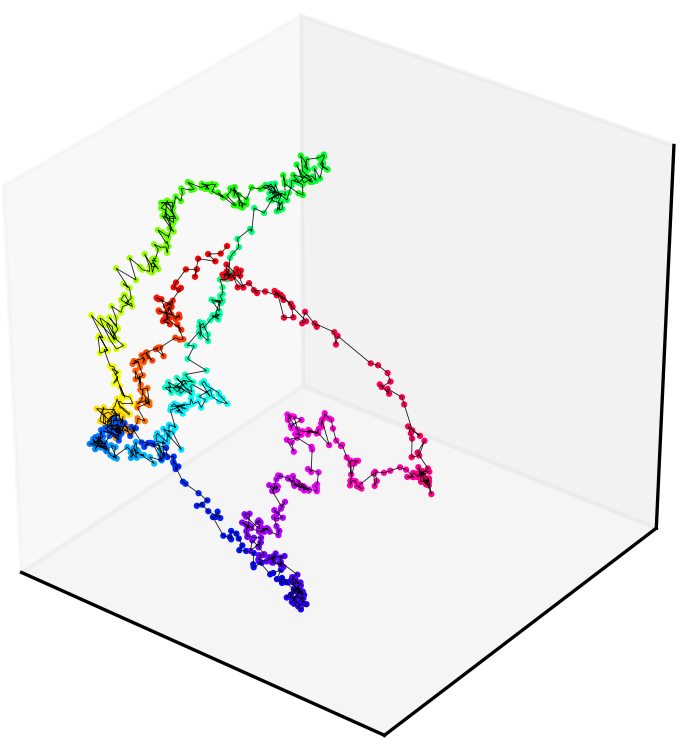
\includegraphics[width=.45\textwidth]{cmp4/cnn8.png}
	}
	\subfigure[Closed self-intersecting trajectory as on figure \ref{fig:model_param}(a)]{
		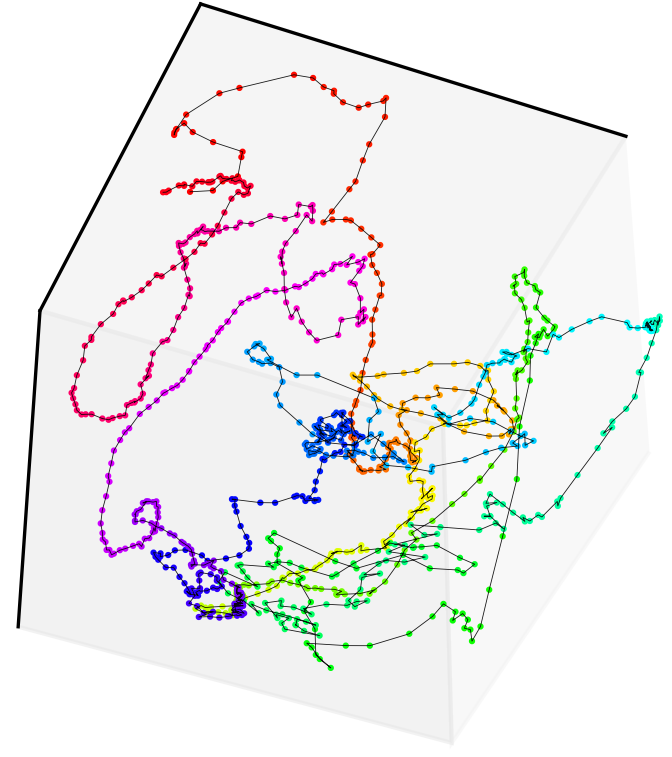
\includegraphics[width=.45\textwidth]{cmp4/cnn82.png}
	}\\
    	\caption{Visualization of first 3 components of 8 dimensional embedding of a validation closed self-intersecting trajectories. Projection is learned by a mixed CNN-FC AE model with next configuration: 16c3-p2-32c3-p2-32c3-p2-16c3-f80-f8.}
    	\label{fig:model_big}
\end{figure}

In this experiment we explored several higher complexity models using different dimensionality of the embedding space: 3, 4 or 8 components. We also experimented with a mixed CNN-FC model, allowing the final layers of the projection (encoder) network to have more complex projection form. We simplicity, we provide a short description of the network architecture in the table \ref{tab:large}. We use next notation to describe network architecture of the encoder: \textit{16c3-p2-32c3-p2-32c3-p2-16c3-f100-f3}. Where first \textit{16c3} corresponds to the first network layer.  \textit{16c3} indicates that layer has 16 convolutional filters of size $3 \times 3$. It is followed by a max-pooling layer $p2$ with stride equal 2. Final layers of the encoder are two fully connected layers  \textit{f100-f3} with 100 and 3 neurons correspondingly. Convolutional layers rely on the ReLU activation function while fully connected layers use logistic sigmoid, as described in section \ref{ss:cnnaec}.

Visual inspection of the embedding even without using dimensionality reduction techniques, showed that trajectory prototype maintains the characteristics actual players path. Namely it intersects itself only in a single place and the time of intersection corresponds to the time of the actual intersection of the trajectory. Yet, the path prototype appear entangled and relatively noisy comparing to previous experiments.

While embedding of the validation trajectory showed continuous form and maintained key intersection, actual model scores are quite low. None of the models was able to provide any improvement in terms of the prediction of the next frame, indicating highly non-linear manifold space at current level of input video discretization.

Models with higher dimensional embedding space showed better performance in terms of maintaining nearest neighbor relation in the embedding space: up to 58\% of $P_{\tau}$ score. They also allowed resulted in reconstruction of the input images. At the same time, predictive score of these models dropped.

Adding another fully connected layer before the last layer of the encoder led to the marginal improvement of all metrics and, more noticeably, of the reconstruction error. Yet, we don't see adding another highly parameterized layer in such a was as a significant advantage.


\subsection{Relevance of the depth information}

In this section we compare effects of the presence or absence of the depth information in the training data. Most of the first person video data comes in form of RGB video channel, that does not contain information about the distance to the objects. In this section we try to asses, how relevant is this information to the task at hand. Results of the experiments for trivial trajectory (see \ref{fig:model_reco}(a)) and an \textit{eight} trajectory (see \ref{fig:model_param}(a)) are shown below.

\begin{table}
\begin{center}
    \begin{tabular}{| l | l | l | l | l |}
      \hline
     Model configuration  &  $P_{L2}$ & $P_{\beta}$ & $P_{\tau}$ & $L_{recoRGB}$ \\ \hline
     Trivial trajectory without depth info		& 0.135 & 0.498 & 0.676 & 63.87 \\
     Trivial trajectory with depth info 		& 0.178 & 0.509 & 0.699 & 64.86 \\ \hline
     "Eight" trajectory without distance information	 	& 0 & 0 & 0 & 86.60 \\
     "Eight" trajectory with distance information		   & 0.476 & 0.778 & 0.236 & 75.49 \\ \hline
    \end{tabular}
\end{center}
  \caption{Comparison of model performance on 2 distinct trajectories depending on presence or absence of the depth information. $L_{recoRGB}$ is calculated only for RGB channels for all models.}
  \label{tab:depth}
\end{table}

Results show, that presence of the depth information in the training data is crucial for the learning the task at hand. Namely, in case of the trivial self-intersecting trajectory depth channel allowed to improve all 3 scores at hand at a low cost of reconstruction error, which is irrelevant to the task at hand. In case of a more complex trajectory model was not able to learn the concept at all without the depth information and projected all points of the trajectory into a single point on the manifold.
